% Author: Dominic van der Zypen
\documentclass[12pt, a4paper]{amsart}
\usepackage{tikz}
\usetikzlibrary{topaths,calc}

\addtolength{\hoffset}{-1cm} % --> Umstellung A4
\addtolength{\textwidth}{2cm}
\addtolength{\voffset}{-1cm}
\addtolength{\textheight}{2cm}

%\mathttheight=645pt
\usepackage{amssymb}
\usepackage{amsthm}
\usepackage{amsfonts}

\newtheorem{lemma}{Lemma}[section]
\newtheorem{theorem}[lemma]{Satz}
\newtheorem{corollary}[lemma]{Korollar}

\theoremstyle{definition}
\newtheorem{definition}[lemma]{Definition}
\newtheorem{remark}[lemma]{Remark}
\newtheorem{example}[lemma]{Example}
\newtheorem{conjecture}[lemma]{Conjecture}
\newtheorem{exercise}[lemma]{Exercise}
\newcommand{\C}{\text{Config}}
\newcommand{\len}{\text{len}}

%-----------------------------------
\begin{document}
\parskip = 2mm
\parindent = 0mm

\begin{center}
    \textbf{\Large ${\bf P}$ vs ${\bf NP}$ \\ for the rigorous mathematician}
\end{center}

\vspace*{3mm}

\begin{center}
Dominic van der Zypen
\end{center}

\section{Introduction}
I have long had an iffy feeling about the formulation of the ${\bf P}$ vs {\bf NP} problem. 
I sort-of know Turing machines, I have a vague concept of what is "a class of problems", 
and I have heard many times that {\bf NP} is the class of problems for which a solution 
can be checked in polynomial time for correctness.

All my ifs-and-buts add to a quite shaky view - and I decided to get to the bottom of 
things and provide a rigorous and (hopefully) mathematically appealing definition of 
Turing machines, languages, and the like. 

%-------------
\section{Configurations}

Let $ \omega$ denote the first infinite ordinal (which can be thought 
of as $ \mathbb{N}$, the set of non-negative integers). Recall that each
$n \in \omega$ is an {\em ordinal}, that is, $0:=\emptyset$ and for $n>0$,
its members are the numbers $ 0,\ldots, n-1$, so $ n = \{0,\ldots,n-1\}$. 
We write $\omega^\omega$ for the collection of all maps $f:\omega \to \omega$.
Members of $\omega^\omega$ are also called {\sl integer sequences}.

Our first 
central concept, the {\bf configuration}, is the mathematical model of the 
notion of the {\bf tape} of the Turing machine, together with the {\bf writing 
head} and the {\bf internal state} of the machine. 


\begin{definition} Let $n \geq 2$ be an integer. Then an {\em $n$-configuration} is a 
    function (also called an {\sl integer sequence}) $c\in \omega^\omega$ with the 
    following properties:
    \begin{enumerate}
        \item $c(0) \in n = \{0,\ldots,n-1\}$,
        \item $c(1) \geq 2$,
        \item $c(k) \in \{0,1,2\}$ for all $k\in\omega\setminus\{0,1\}$, and
        \item $c$ is eventually constant with value $2$. (This means
            that there is $N\in \omega$ such that $c(k) = 2$ for all $k\in \omega$
            with $k\geq N$.)
    \end{enumerate}
\end{definition}

Next, we illustrate and explain the meanings of the entries of $c$ in detail:

\vspace*{1mm}

%--- bildli ---
\begin{center}
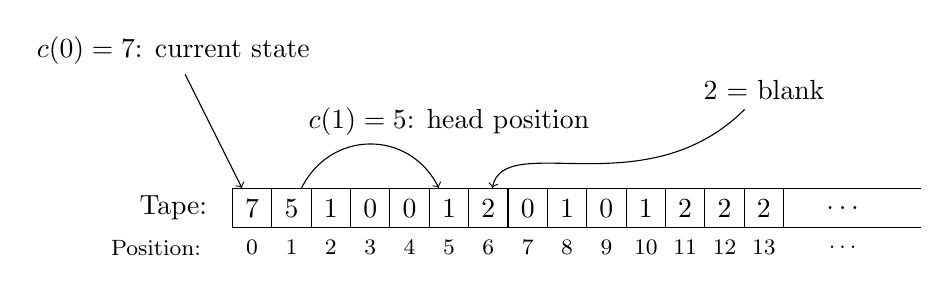
\begin{tikzpicture}[
   box/.style={rectangle,draw,minimum width=0.5cm,
    minimum height=0.5cm,inner sep=+0.1cm}
    ]

    % Boxes:
    \node at (0,1) {Tape:};
    \node[box] at (1,1) (h0) {7};
    \node[box] at (1.5,1) (h1) {5};
    \node[box] at (2,1) (h2) {1};
    \node[box] at (2.5,1) (h3) {0};
    \node[box] at (3,1) (h4) {0};
    \node[box] at (3.5,1) (h5) {1};
    \node[box] at (4,1) (h6) {2};
    \node[box] at (4.5,1) (h7) {0};
    \node[box] at (5,1) (h8) {1};
    \node[box] at (5.5,1) (h9) {0};
    \node[box] at (6,1) (h10) {1};
    \node[box] at (6.5,1) (h11) {2};
    \node[box] at (7,1) (h11) {2};
    \node[box] at (7.5,1) (h11) {2};
    \node at (8.5, 1) (h16) {$\ldots$};

    % Positions:
    \node at (-0.22,0.5) {\footnotesize{Position:}};
    \node at (1,0.5) {\footnotesize{0}};
    \node at (1.5,0.5) {\footnotesize{1}};
    \node at (2,0.5) {\footnotesize{2}};
    \node at (2.5,0.5) {\footnotesize{3}};
    \node at (3,0.5) {\footnotesize{4}};
    \node at (3.5,0.5) {\footnotesize{5}};
    \node at (4,0.5) {\footnotesize{6}};
    \node at (4.5,0.5) {\footnotesize{7}};
    \node at (5,0.5) {\footnotesize{8}};
    \node at (5.5,0.5) {\footnotesize{9}};
    \node at (6,0.5) {\footnotesize{10}};
    \node at (6.5,0.5) {\footnotesize{11}};
    \node at (7,0.5) {\footnotesize{12}};
    \node at (7.5,0.5) {\footnotesize{13}};
    \node at (8.5, 0.5) {\footnotesize{$\ldots$}};

    % ... etc-lines:

    \draw (7.5,1.25) -- (9.5,1.25);
    \draw (7.5,0.75) -- (9.5,0.75);

    % blank / head / state

    \node at (0, 3) (state){$c(0) = 7$: current state};
    \node at (3.5, 2.1) (head){$c(1) = 5$: head position};
    \node at (7.5, 2.5) (blank){$2$ = blank};

    % arrows

    \draw[->] (state) -- (h0); % state -> 0 arrow
    \draw[->] (h1) .. controls (2,2) and (3,2) .. (h5);
                     % pointer arrow from 1 to 5
    \draw[->] (blank) .. controls (6,1) and (4.2,2) .. (h6);
                     % blank arrow

\end{tikzpicture}
\end{center}

%--- /bildli ---

\vspace*{1mm}

\begin{itemize}
    \item $c(0)\in n$ represents the {\em state} of the possible $n$ 
        states $\{0,\ldots,n-1\}$ of the configuration. States 0 and 1 
        (stored in the first cell, $c(0)$) have a special meaning: 
        $0$ = {\em reject}, $1$ = {\em accept}.
    \item $c(1) \geq 2$ represents the position of the {\em read/write head}
        of the configuration.
    \item We interpret $2$ as being the {\em blank} symbol. The {\em value} 
        symbols are 0 and 1. The blank symbol 2 can be used to separate "input strings" 
        consisting of 0,1. Every configuration is eventually blank (=2).
\end{itemize}

We let $\C(n)$ be the collection of $n$-configurations. Note that
whenever $n\leq n'\in \omega$ and $n\geq 2$, we have $\C(n)\subseteq \C(n')$.

%--------------
\section{Turing machines}

\begin{definition}
A {\em Turing machine} is a tuple $M=(n, \delta)$ where $n\in\omega,
    n\geq 2$ and $\delta: n \times \{0,1,2\} \to n \times \{0,1,2\} \times
    \{-1,1\}$ is a function with following property: 
    \begin{quote} if 
    $q \in \{0,1\}$\footnote{recall that 0,1 are special states with 
        the meanings
    $\{${\em reject, accept}$\}$, respectively.}
     and $b\in \{0,1,2\}$, then $\delta(q,b) = (q,b,-1)$.
    \end{quote}
\end{definition}

The interpretation of this is that $\delta$ gets constant
whenever an {\em accept} or {\em reject} state has been reached.

If $\delta(q,b) = (q', b', s)$ for $q,q'\in Q, b,b'\in \{0,1,2\}$ and 
$ s\in \{-1,1\}$
we write
\begin{itemize}
    \item $\mathtt{nextstate}(q,b) = q'$,
    \item $\mathtt{output}(q,b) = b'$, and
    \item $\mathtt{step}(q,b) = s\in\{-1,1\}$. 
\end{itemize}
The function $\delta$ is called the {\em transition function} and can 
be looked at as the {\sl clockwork} of the Turing machine.

%------------------
\section{Synthesis: combining configurations and Turing machines}

\begin{definition}
    If $M=(n,\delta)$ be a Turing machine, then $M$ induces a {\em configuration
    map} $${\frak C}_M: \C(n)\to \C(n)$$ in the following way. If $c\in \C(n)$,
    then we define ${\frak C}_M(c): \omega \to \omega$ by

    \begin{itemize}
        \item ${\frak C}_M(c)(0) = \mathtt{nextstate}(c(0), c(c(1)))$
            \footnote{$c(0)$ is the current state 
            in the set of possible states $\{0,\ldots,n-1\}$, and $c(1)$
            is the position of the read/write head, and finally $c(c(1))$ is the
            {\bf value} of the cell at the head.}
        \item ${\frak C}_M(c)(1) = 
            \max\big\{2, c(1) + \mathtt{step}(c(0), c(c(1)))\big\}$,
            \footnote{$\mathtt{step}(c(0),c(c(1)))\in\{-1,1\}$.}
        \item ${\frak C}_M(c)(c(1)) = \mathtt{output}(c(0), c(c(1)))$, and
            \footnote{so the output created by the transition function $\delta$ gets
            inserted at the head position $c(1)$.}
        \item ${\frak C}_M(c)(x) = c(x)$ for all $x\in\omega \setminus \{0,1,c(1)\}$. 
    \end{itemize}
    So we have ${\frak C}_M(c) \in \omega^\omega$, and it easy to check that
    ${\frak C}_M(c) \in \C(n)$. 
\end{definition}

%------------------------------------
\section{Run time and worst-case run time}

If $X\neq \emptyset$ is a set and $f:X\to X$, we define inductively for any $x\in X$:
\begin{itemize}
    \item $f^{(0)}(x) = x$, and
    \item $f^{(n+1)}(x) = f\big(f^{(n)}(x)\big)$.
\end{itemize}

For the remainder of this section, fix $n\geq 2$.

\begin{definition}
    If $M$ is an $n$-Turing machine and $c\in \C(n)$, then we consider
    the set 
    $${\mathcal T}_M(c) = \big\{n\in\omega:{\frak C}_M^{(n)}(0) \in 
        \{0,1\}\big\}.\footnote{This is the set of iterations $n$
        such that the state stored in the first cell is 0 (reject)
        or 1 (accept).}$$
    \begin{enumerate}
        \item If ${\mathcal T}_M(c)\neq\emptyset$, we 
            say that $M$ {\em terminates}
        on constellation $c$. 
    \item The {\em run time} of $M$ on $c$ defined by 
        $t_M(c) = \min {\mathcal T}_M(c)$ if $M$ terminates on $c$,
            and we set $t_M(c) = \infty$ otherwise.
    \item If there is $n\in \omega$ with ${\frak C}_M^{(n)}(0)=0$, then
        $M$ is said to {\em reject} $c$.
    \item If there is $n\in \omega$ with ${\frak C}_M^{(n)}(0)=1$, then
        $M$ is said to {\em accept} $c$.
    \item We define the
        the {\em language accepted by $M$} by $$L(M) = \{c \in \C(n): M
    \text{ accepts } c\}.$$
    \end{enumerate}
\end{definition}

For the {\em worst case run time} we need the notion of the
length of a configuration. Note that every configuration is
eventually constant $2$.

\begin{definition} If $c\in \C(n)$, the the {\em length} of $c$
    is defined by $$\len(c) = \min\{N\in\omega\setminus\{0,1\}: c(x) = 2
   \text{ for all } x\geq N\} - 2.$$
\end{definition}

(It is a bit aesthetically displeasing that one has to do this
$\omega\setminus\{0,1\} [\ldots] -2$ trick. This is because the 
first two cells $c(0), c(1)$ of each configuration $c$ have special meanings,
and the input starts at $c(2)$.)

\begin{definition}
    If $M$ is an $n$-Turing machine and $\ell\in\omega$ then 
    we define the {\em worst case run time} to be 
    $$T_M(\ell) = \sup\{t_M(c): c \in \C(n)\text{ and } 
    \len(c) = \ell\}\in \omega\cup\{\infty\}.$$ We say 
    that $M$ {\bf runs in 
    polynomial time} if there are positive integers $j, k$ 
    such that for all $\ell \in \omega$ we have $T_M(\ell) \leq
    \ell^j + k.$
\end{definition}

%--------------------
\section{The class {\bf P}}

$\mathbf{P} = \big\{L\subseteq \omega^\omega : $ there is an integer $n\geq 2$
and an $n$-Turing machine $M$ \\ \hspace*{27mm} such that 
$L=L(M)$ and $M$ runs in polynomial time$\big\}$.
\end{document}
